%More details on electron reconstruction can be found in Ref.~\cite{ElectronLegacy}. 
Both of electron and photon are important ingredients of the analysis upon which the dissertation is based. Both interact electromagnetically and can be reconstructed and identified at CMS very efficiently which is also the requirement physics analyses. Photon being chargeless deposits its energy only in the electromagnatic calorimeter (ECAL), as described in Section. \ref{cms:ecal}, ~ leaving no track in the ITS of CMS. On the other hand, electrons leave tracking information in the ITS and well as in the ECAL. A schematic diagram of the behavior of photon and electron as they fly out of the interaction point from ITS to ECAL is shown in the Figure \ref{fig:ele_photo}.

\begin{figure}[!htb]
\vspace*{0.3cm}
\begin{center}
%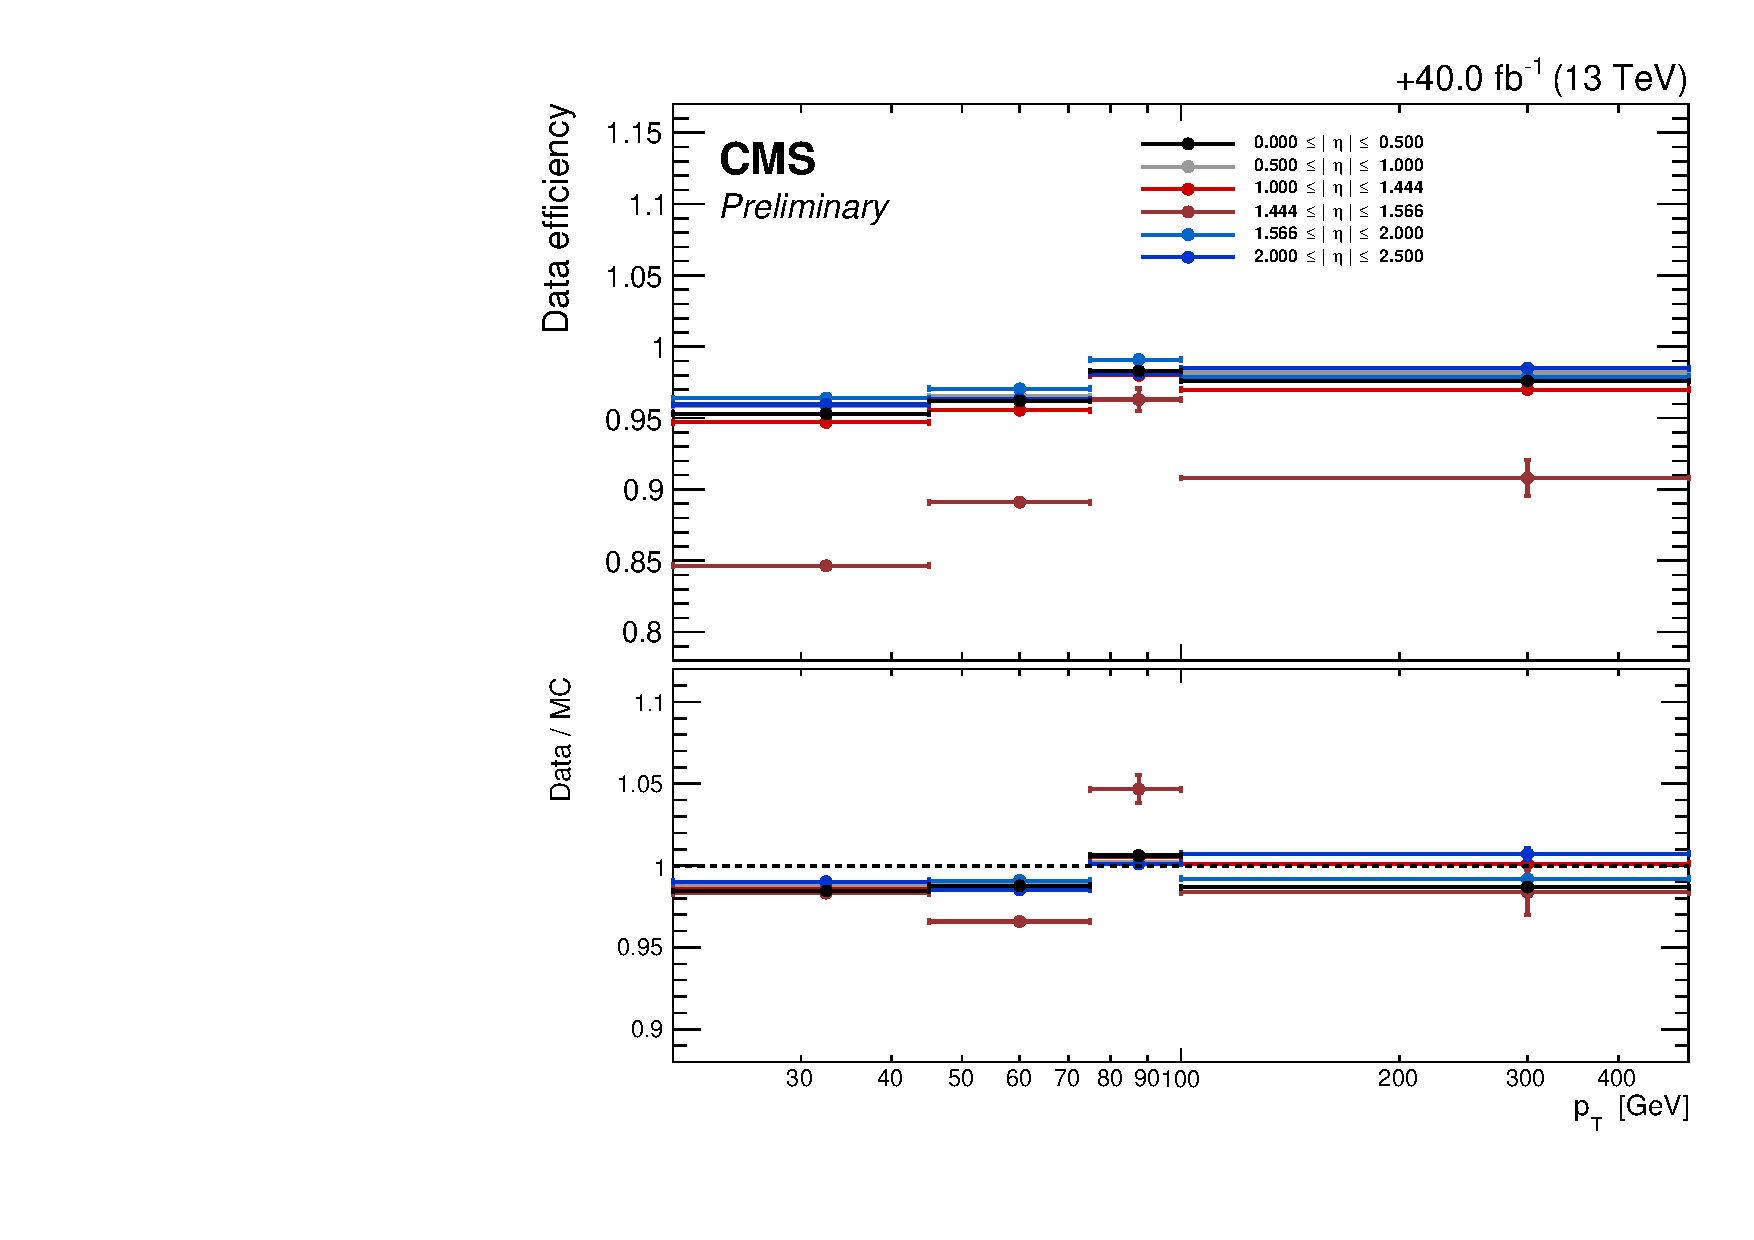
\includegraphics[width=0.4\textwidth]{Figures/Electrons/ErecoPt}
%\includegraphics[page=2, width=0.4\textwidth]{Figures/Electrons/ErecoEta}\\
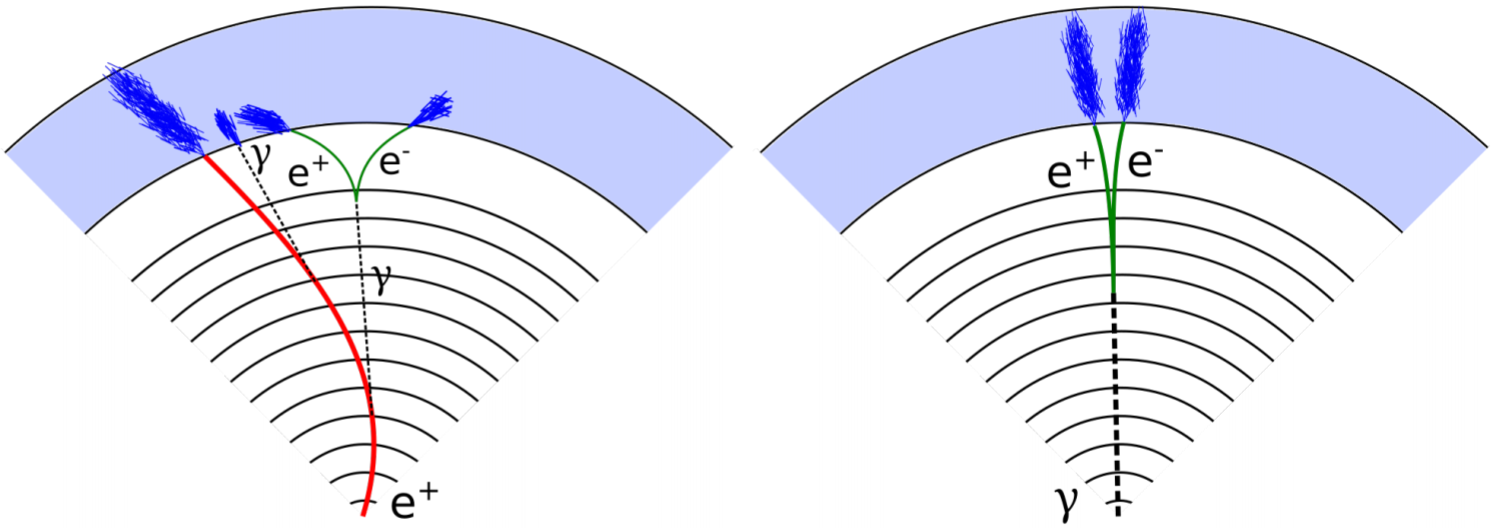
\includegraphics[width=0.9\textwidth]{Figures/ele_photo.png}
%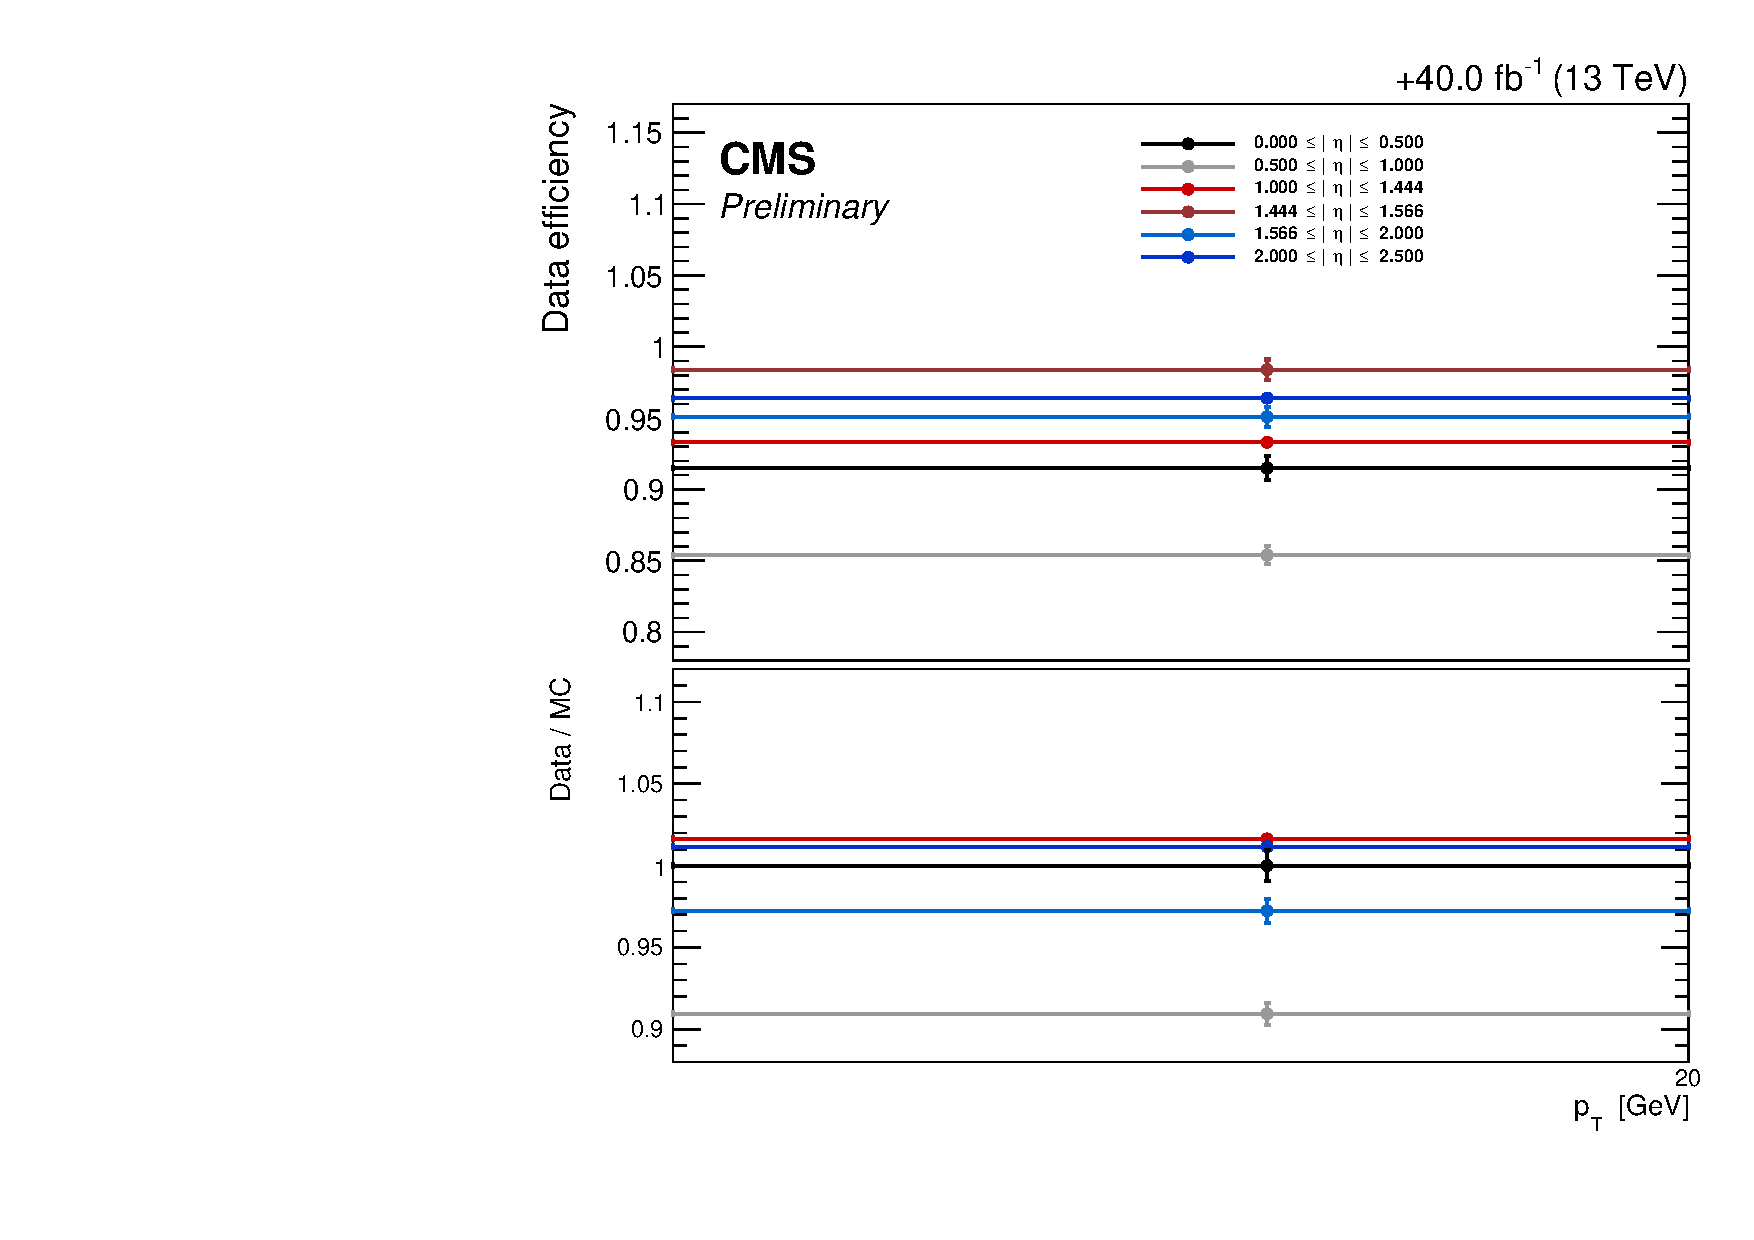
\includegraphics[width=0.4\textwidth]{Figures/Electrons/ErecoEta_lowPt}
\end{center}
	\caption{Pattern of positron (photon) to the detector shown left (right).}
\label{fig:ele_photo}
\end{figure}

There are many ways to identify the true or uncoverted photons e.g. by using:
\begin{itemize}
	\item Tracker, ECAL and HCAL isolation
	\item Hadronic to electromagnetic ratio
	\item $R_{9}$~ ratio
\end{itemize}

Electrons can be reconstructed and identified when a supercluster is associated to a track in the silicon detector. 
For track reconstruction of electron, as described in Section \ref{sec:track_reco}, ECAL based seeding is efficient for $\pt>10$; however, for lower $\pt$ Tracker based seeding (that makes use of boosted decision tree (BDT) for preselection of tracker clusters) is more efficient.  
$\pt$ of the electron is measured from these tracker tracks produced when it pass through it. Being charged particle, it has curved track under the influence of superconducting magnet due to which it radiates to photons. Therefore, Gaussian Sum Filter (GSF) algorithm, which takes into account the bremsstrahlung losses, is used to reconstruct the track.

Preselection of the electron candidates is made through loose cuts on track-cluster matching observables. This done to maintain highest possible selection efficiency of electrons and to reject QCD background significantly. For the analysis, electrons are subjected to have $p^e_T >$ 7 GeV within $|\eta^e| <$ 2.5, and satisfy a loose primary vertex 
constraints on longitudinal and transvers components of impact parameter $viz.$ $d_{xy} < 0.5$ cm and $d_z < 1$ cm respectively.
Such electrons are called {\bf loose electrons}. Details of electron reconstruction can be explored in Ref.~\cite{ElectronLegacy}.

The data-MC discrepancy is corrected using scale factors as is done for the electron selection with data efficiencies measured through technique outlined later (see Section \ref{sec:eleEffMeas}). 
These studies for reconstructions are carried out by the E/gamma Physics Object Group (EGM POG)\footnote{The charge of the EGM POG is to study, develop, characterize and validate the tools to identify and reconstruct electrons and photons using all the information available from the CMS detector, both for the offline analysis and for the online event selection (HLT)}.

The electron reconstruction scale factors are shown Figure \ref{fig:ele_rec_scale_factors} and are applied as a function of electron $\pt$ and super cluster $\eta$.

\begin{figure}[!htb]
\vspace*{0.3cm}
\begin{center}
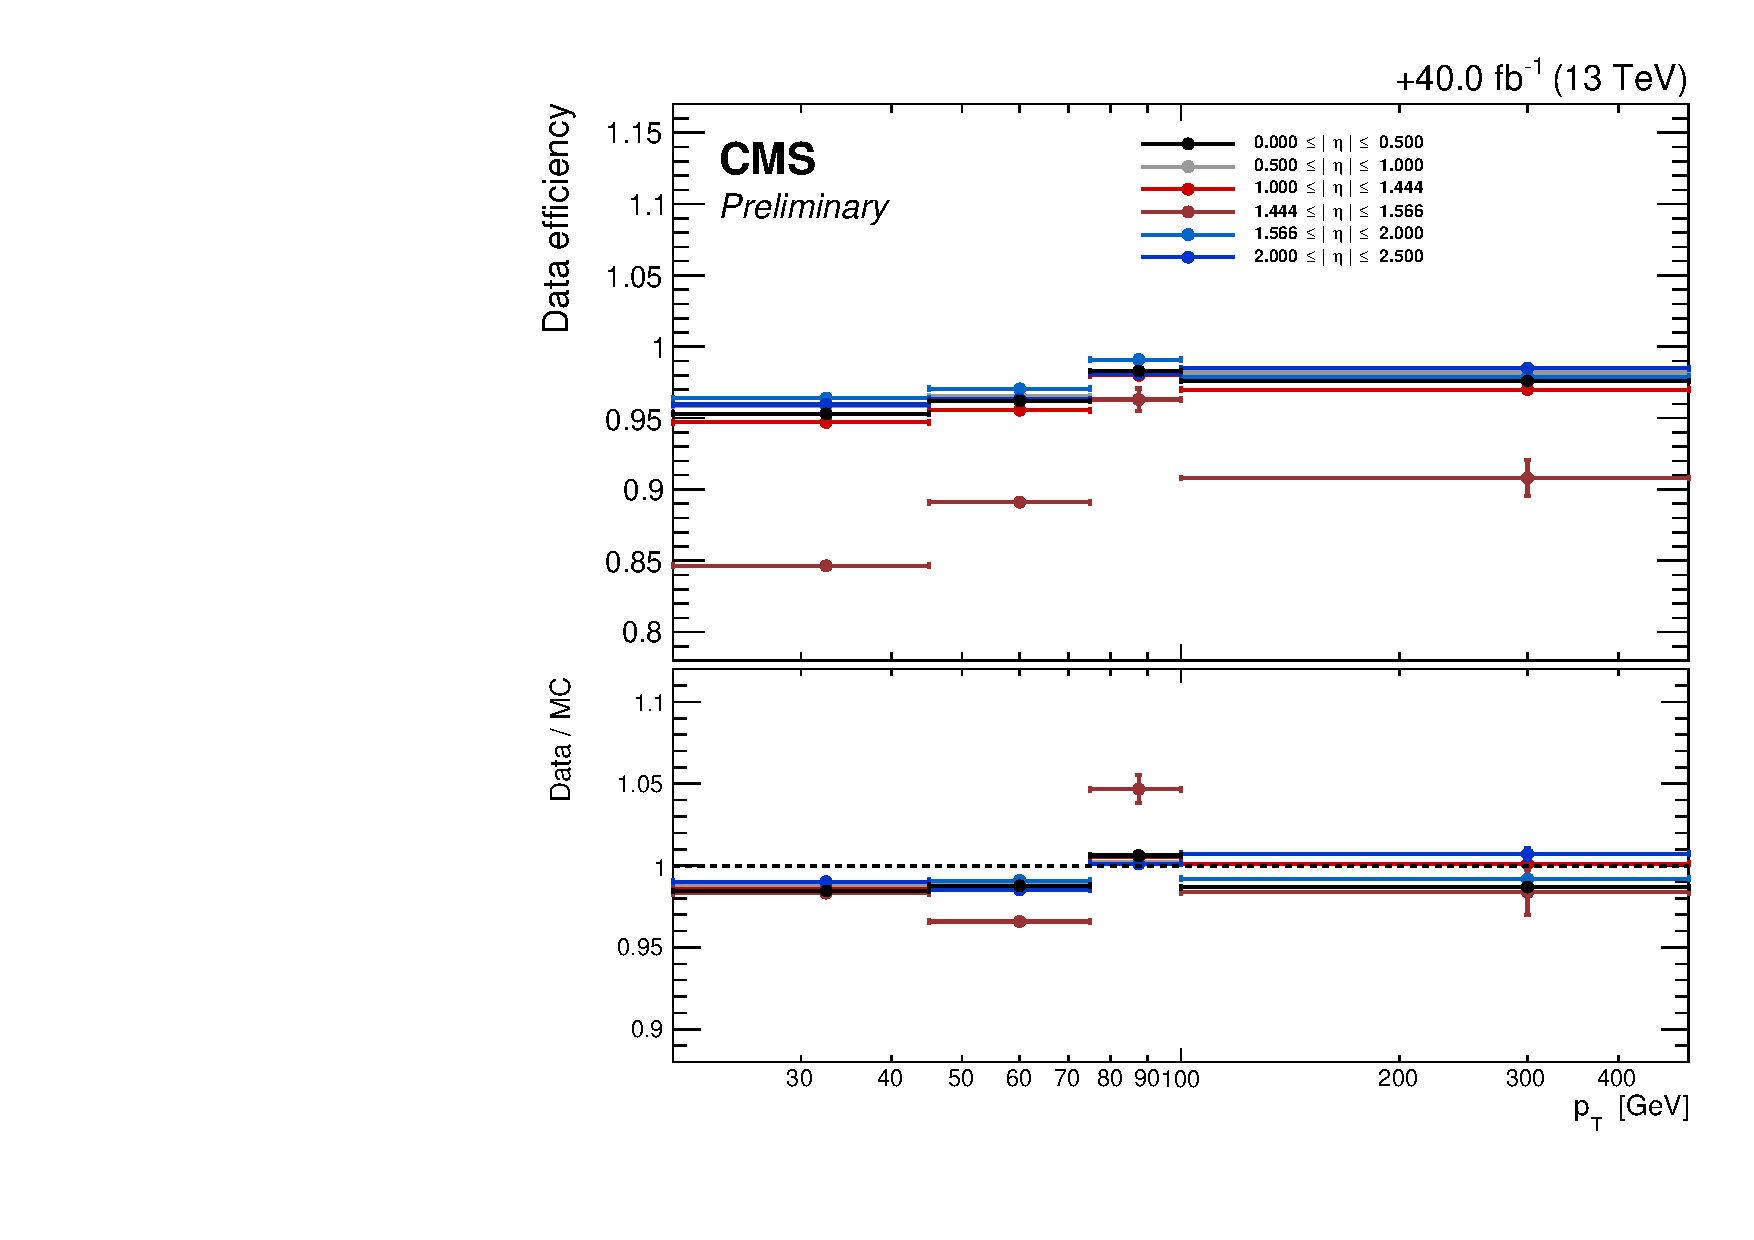
\includegraphics[width=0.48\textwidth]{Figures/Electrons/ErecoPt}
\includegraphics[page=2, width=0.48\textwidth]{Figures/Electrons/ErecoEta}\\
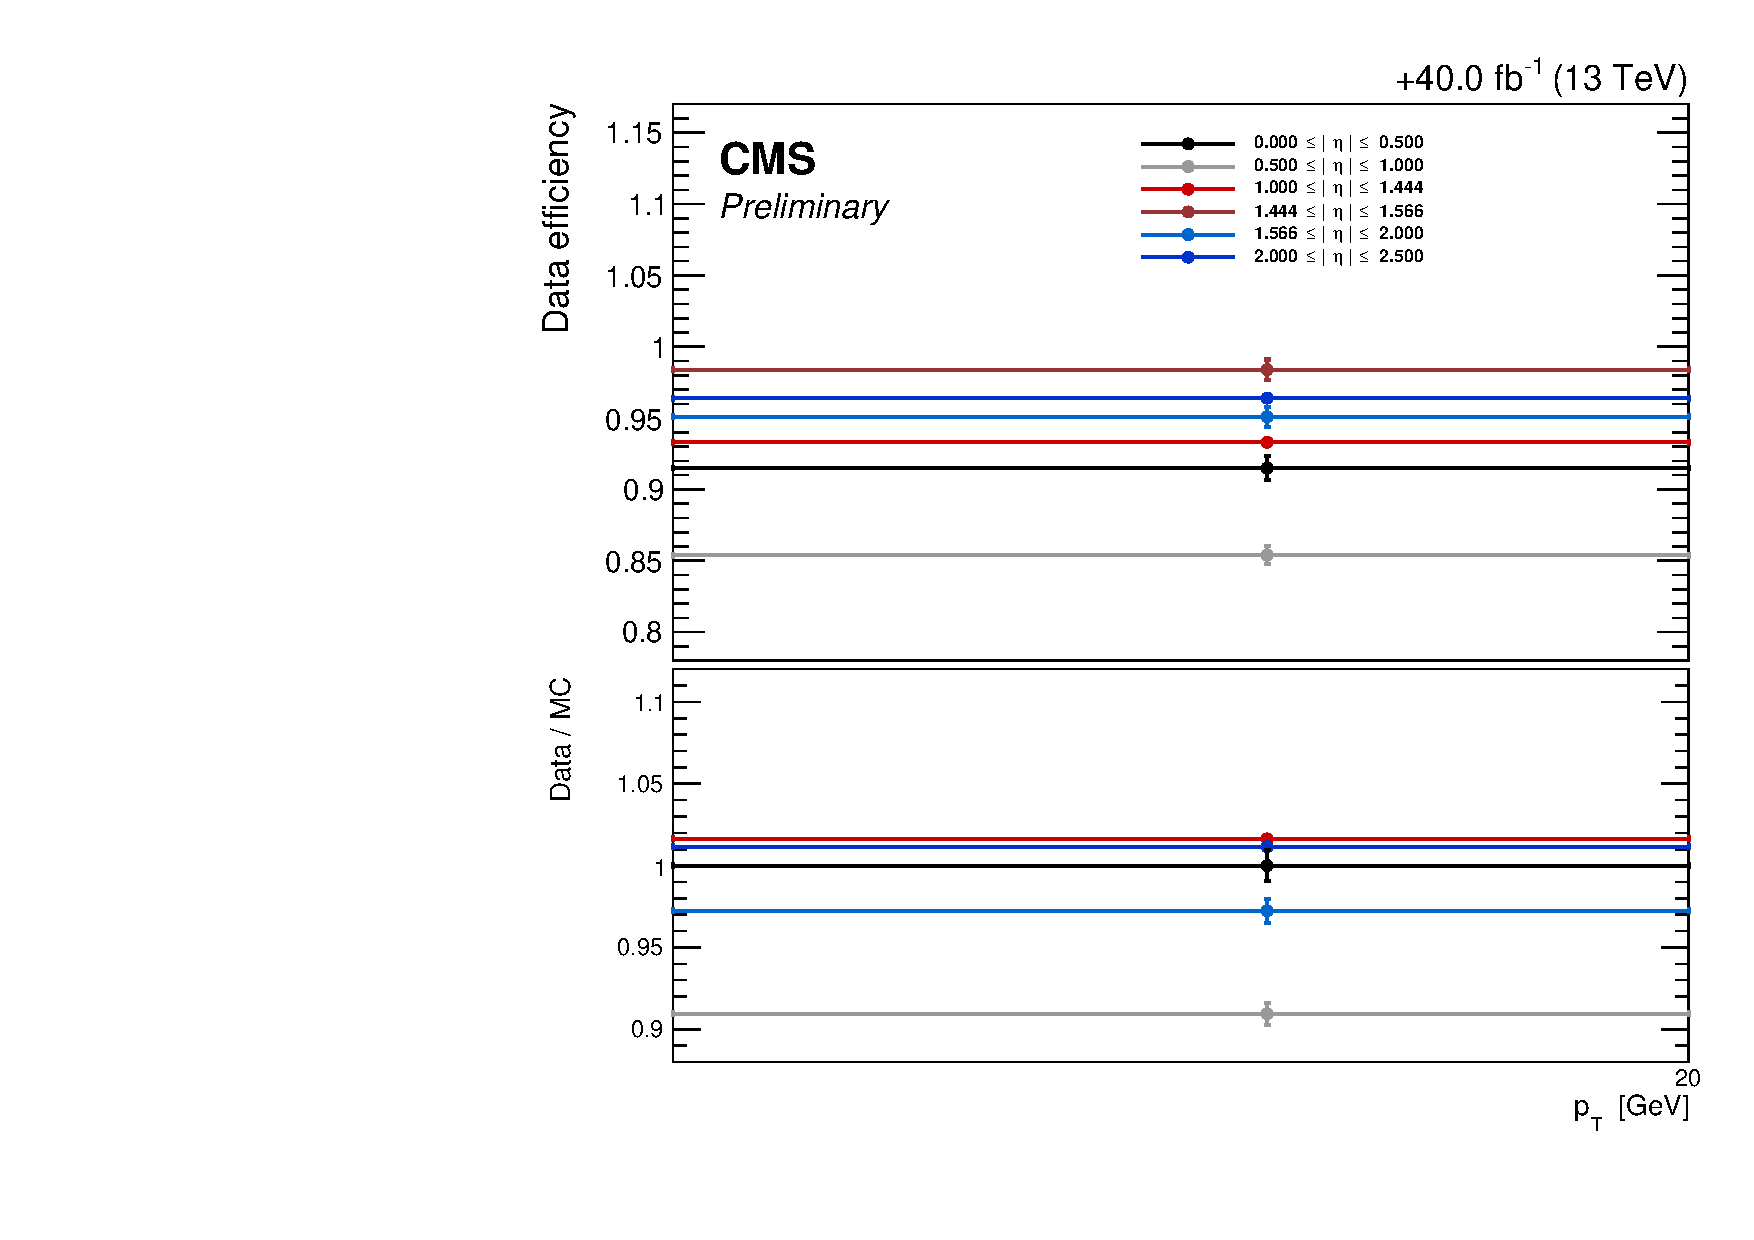
\includegraphics[width=0.48\textwidth]{Figures/Electrons/ErecoPt_lowPt}
%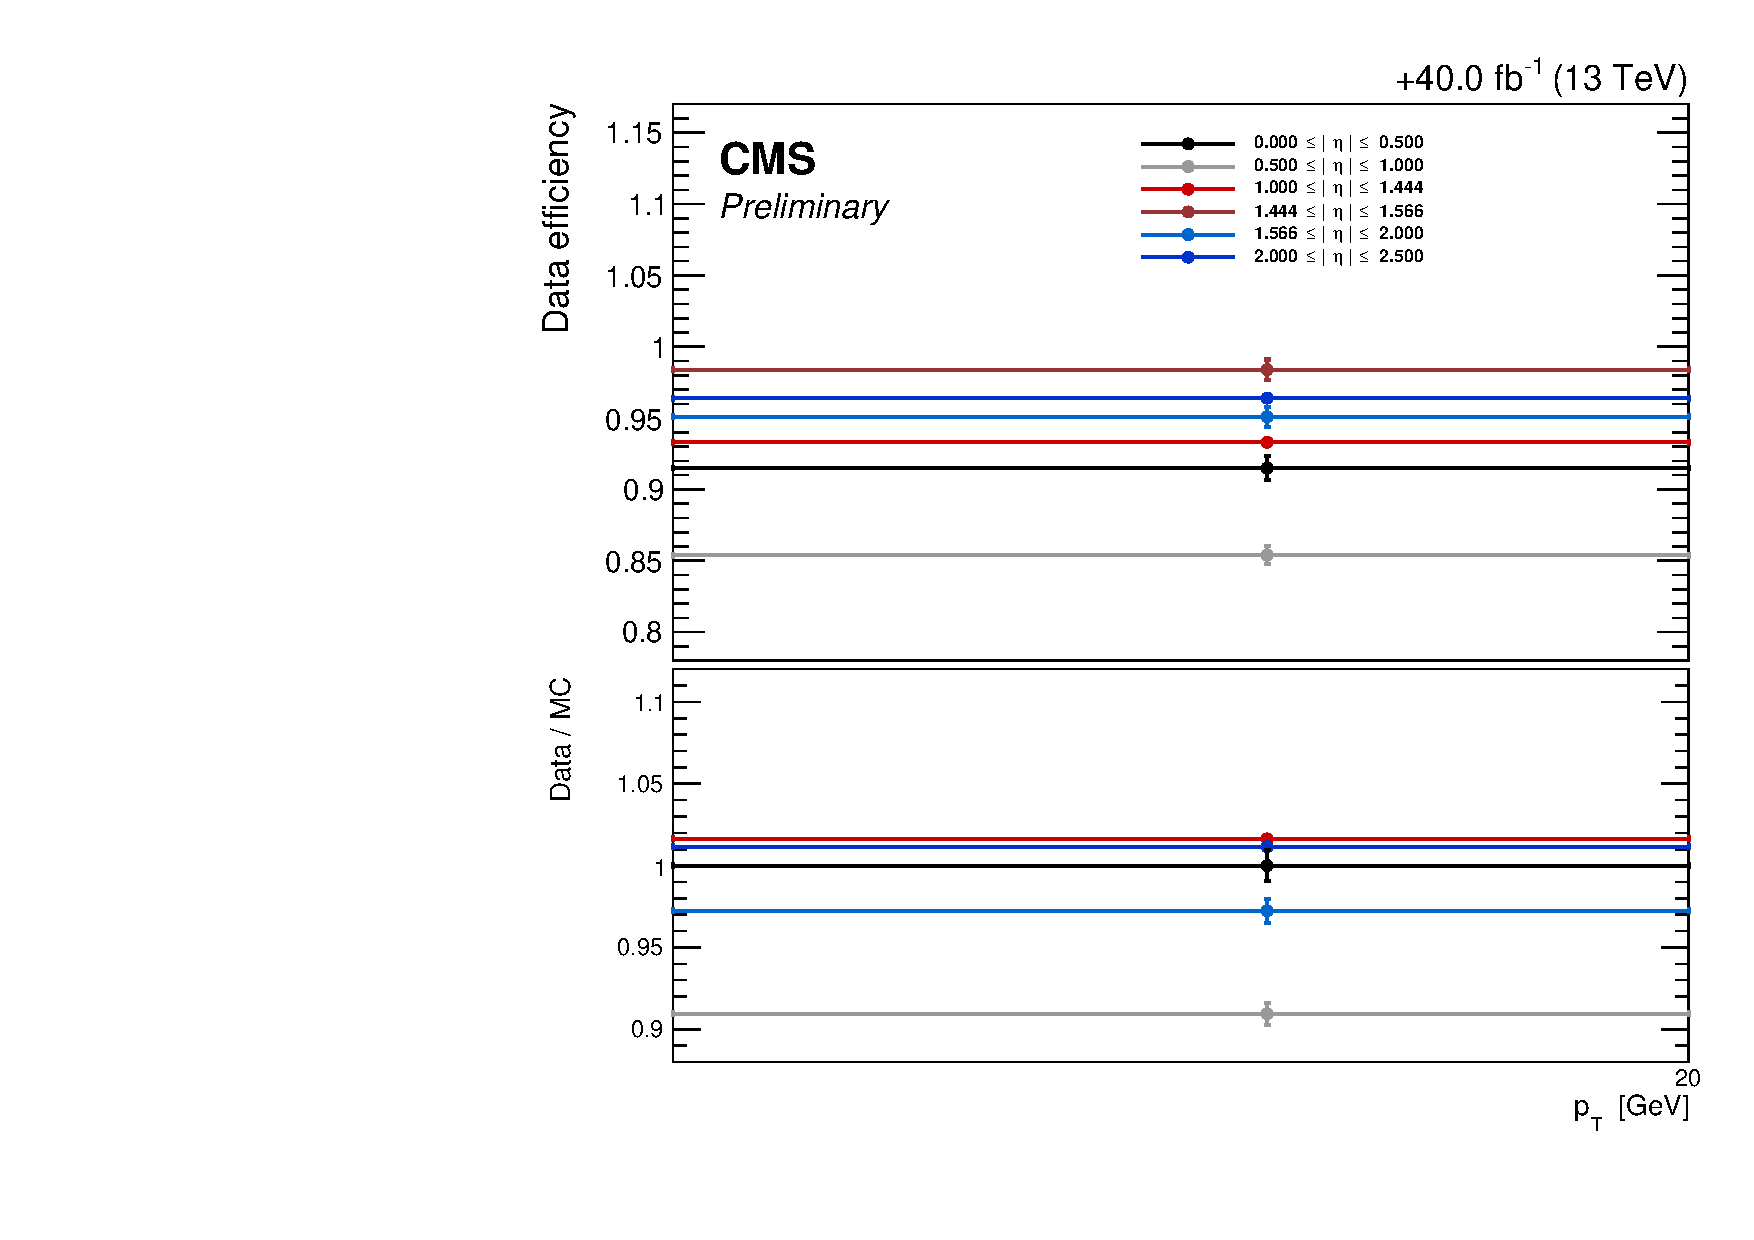
\includegraphics[width=0.4\textwidth]{Figures/Electrons/ErecoEta_lowPt}
\end{center}
\caption{Reconstruction efficiencies of electron in data versus $p_T$ (left), $\eta$ (right) for electrons having $\pt > 20 \GeV$ (top) and $\pt < 20 \GeV$ (bottom) with corresponding data/MC scale factors as provided by the EGM POG.}
\label{fig:ele_rec_scale_factors}
\end{figure}


